
\subsection{History and Related Concepts}\label{sec:Theory}
The term \emph{glyph} is originated from Greek word, \emph{glyph\={e}}, meaning carving. Since the 16th century, its uses in English have been much associated with etymology, archaeology, topography and graphonomics. Although its contemporary use in the context of multivariate visualization may seem rather different, they share many interesting attributes, such as being ``small'', being ``visual'', having ``meaning'', requiring ``learning'', and often being ``metaphoric''. It is thus interesting to study briefly the related history and concepts.    

%\subsection{Definitions and Fundamental Concepts}
%Definition of what a sign is and its role as a communication mean, e.g., Marcus's glossary, 
%Definition of semeiotic
%\\Peirce's Semiotic: Definition of sign, interpretant, immediate object, dynamical object.
\begin{figure*}[!h]
  \centering
  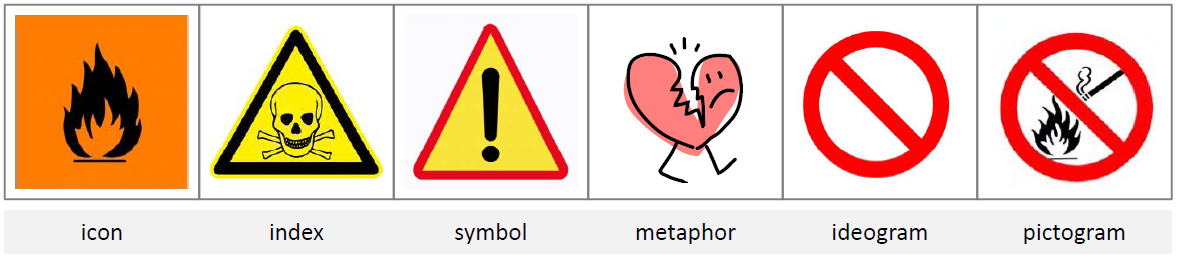
\includegraphics[width=162mm]{images/related-work-glyphs/Signs.png}
  \caption{In philosophy, language studies and psychology, signs may take one of the three forms, icon, index and symbol. In many contexts, terms such as visual metaphor, ideogram and pictogram are also used to denote subclasses of signs.\label{fig:Signs}}
\end{figure*}


\subsection{A brief history of the study of signs}
Signs in terms of indices, icons and symbols (Figure~\ref{fig:Signs}) are all different aspects of a similar unit of knowledge representation, which
has been used as a fundamental concept in trade, commerce and industry from early days to present.
Symbolism has played an important part in the development of human culture, especially as a form of communication. %(see Figure~\ref{fig:caves}).
The Paleolithic Age, around 18,000 BC, has given us hundreds of examples in the form of cave paintings. 
The Neolithic Age instead provides the first forms of pre-writing symbols used for communication: the Petroglyphs, images incised in rock \emph{petra} (meaning ``stone'') + \emph{glyphein} (meaning ``to carve'') . Tribal societies continue 
to use this form of symbolic writing even in current times. 
%\begin{figure}[!ht]
% \centering
% 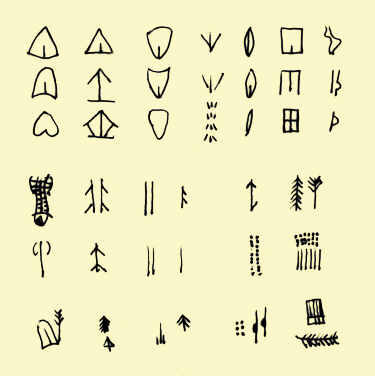
\includegraphics[width=2.0in]{images/related-work-glyphs/representing morphemes, and ideograms, which images/related-work-glyphs/FranceSymbols.jpg}
% \caption{Symbolic representation, Australia Hunter Valley National Park.}\label{fig:caves}
%% \caption{Symbolic representation, Australia Hunter Valley National Park.}\label{fig:caves}
%\end{figure}
 
Examples of pictograms can be easily found today. Interesting examples are the Pub and Inn signs found in England, Europe and North America. After an edict from King Richard II in 1393 that required all alehouses to post a sign they soon became a method of identifying and promoting themselves to the official ale tasters and the public. These signs still remain a tradition often exposing creative and unusual but always metaphoric. The use of symbols and signs has traversed human history for generations, due to their cross-cultural expressive power. Signs and symbols are fundamental means for communication transcending cultural boundaries. With the advent of the computer era, icons have become one of the most popular means of conveying messages. In the early 1980s the CHI community~\cite{Blattner1989,Bly1982,Gayer1989} investigated the use of sounds in associations with visual display to create a new type of multi sensory signs: the ``earcons''. 
Today the use of icons, with added sophisticated features such as animations and sounds, is now pervasive throughout most media platforms.  
As highlighted by Marcus~\cite{Marcus2003} specialised communities such as health and medicine, finance and banking, travel and transportation, and education
and training, already possess widespread and sophisticated proprietary visual sign systems.
The power of expression inherent to visual sign systems is appealing to media, technology and information visualization alike. 
The challenge relies on the development of well-designed sign systems. 

\begin{figure}[!h]
 \centering
 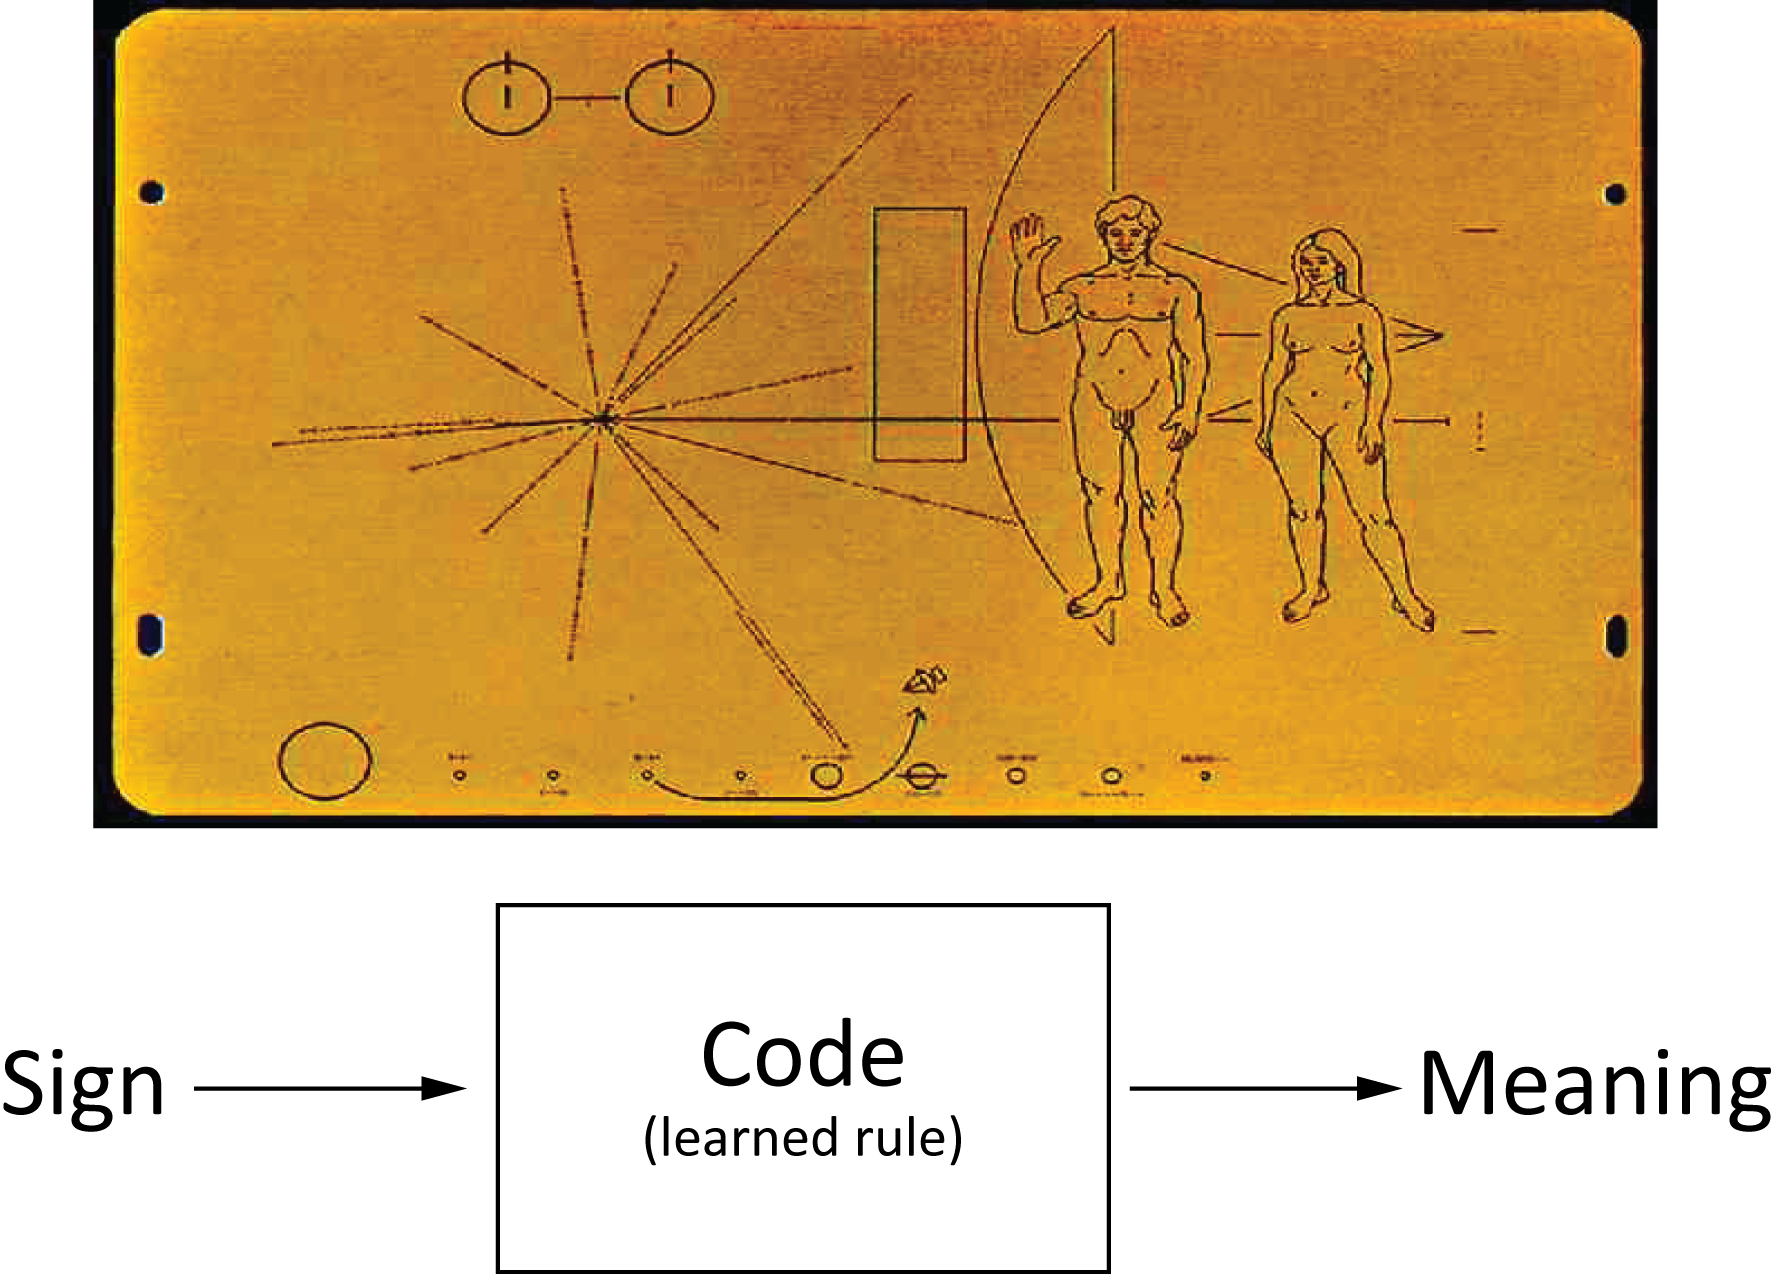
\includegraphics[width=.45\textwidth]{images/related-work-glyphs/SignCode.png}
 \caption{The Pioneer 10 Spacecraft 1972 Plaque.}\label{fig:plaque}
% 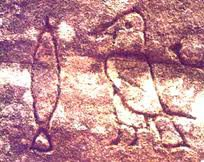
\includegraphics[width=2.0in]{images/related-work-glyphs/caves.jpg}
% \caption{Symbolic representation, Australia Hunter Valley National Park.}\label{fig:caves}
\end{figure}
\subsubsection{Functional Space}
According to Peirce~\cite{Peirce1902}'s theory of signs all modes of thinking depend on signs. Signs act as mediators between the external world of objects and the internal world of ideas.  
A sign in itself is a \emph{stimulus pattern} associated with a \emph{meaning}. Depending on \emph{how} the meaning is associated 
with the pattern (or object) a sign can be classified as either an icon, an index or a symbol. 
The icon, index and symbol triad represents the different relationship between the sign and its object.
Icons (such as pictures, images, models, or diagrams) represent a sign that itself resembles the qualities of the object it stands for (\emph{physical correlation}). Indexes are defined by some sensory feature (such as a clock, thermometer, fuel gauge, or medical symptom) and therefore represent a sign which demonstrates the influence of its object (\emph{space and time correlation}). Symbols (such as a trophy, medal, receipt, diploma, monument, word, phrase, or sentence) represent a sign which is interpreted as a reference to its object. For this reason, symbols are the only type of sign which do not require any physical, space or time correlation between the sign and its meaning (\emph{metaphysical correlation}).  

Codes provide the framework within which signs assume a meaning. A symbol, for example, is a sign where the function is a conventional rule (or coding) and is dependent only on a process of interpretation (Figure~\ref{fig:plaque}).

\subsubsection{Icons} The functional domain of icons is comprised of: images, metaphors and diagrams. These three items all share topological similarity with the object they are related. Images share sensory qualities, 
diagrams share relational and structural qualities, while metaphors elicit the representative character of an object by building a parallelism with something else~\cite{Johansen2002}. The typology of signs can be described based on the different ways a sign refers to its object~\cite{Peirce1955}.
Indices require the existence of the object they are a sign of, symbols require an interpreter; while icons require neither object nor interpreter.
A Euclidean diagram for example, is made up of streaks of pencil lead that represent a geometric line even though the latter ``has no existence''~\cite{Peirce1902}.


\subsubsection{Indices} The functional domain of indices is comprised of: tracks, symptoms and designations~\cite{Johansen2002}. The three types of index represent abstractions that rely on a physical cause/effect relation which is not necessarily simultaneous with the object to which they relate to. Despite simultaneously not being a constraint, an index cannot be a sign without its object (e.g smoke is a symbol/sign of fire).

\subsubsection{Symbols} The functional domain of symbols is comprised of  all abstractions which rely on a code conventionally used in order to determine meaning. Examples of symbols are languages, mathematical symbols and alphanumeric characters on a computer keyboard. Symbols as signs need an interpreter but do not require any space or time correlation with the object they are a sign of, therefore a symbol represents the only type of sign which: a) can be easily removed from its context; and b) is closely associated with large sets of other words. 
%\textbf{TODO: Add a picture with the symbol icon index triad maybe examples...}



\subsubsection{Codes}
The Pioneer 10 plaque (Figure~\ref{fig:plaque}) represents an attempt at communication with alien beings via a ``pictorial message'' including all three type of signs previously described (e.g. icons, indices and symbols) and it is an exemplar testimony of the importance of what semioticians call codes.
Coding is one of the fundamental concepts in semiotics and represents a deterministic functional relation between two sets of entities,  namely: a signifier and a signified.
Reading an image, like the reception of any other message, is dependent on prior knowledge of possibilities (signifier); we can only recognise what we know (signified).
It is this information alone that enables us to separate the code from the message.
%Semiotic codes are procedural systems of related conventions for correlating signifiers and signifieds in certain domains. 
Related to sign, it is possible to distinguish between three main kind of codes~\cite{Chandler2002}: social codes, textual codes and interpretative codes. % (perceptual and ideological). 


\paragraph{Social Codes.} 
All semiotic codes can be broadly classified as social codes, however within our classification we refer to social code in their narrow sense concerning implicit or explicit 
social agreements and behaviours as in: 
\begin{itemize}
\item verbal language: phonological, syntactical, lexical, prosodic and paralinguistic subcodes;
\item bodily codes: bodily contact, proximity, physical orientation, appearance, facial expression, gaze, head nods, gestures and posture;
\item commodity codes: fashion, clothing and cars;
\item behavioural codes: protocols, rituals, role-playing and games.
\end{itemize}

\paragraph{Textual Codes.} 
Next to social codes and interpretative codes, textual codes  represent one of the majour groups of codes. According to Chandler's classification~\cite{Chandler2002}, textual codes relate to our knowledge and often act as vehicles to represent reality (representational codes). Examples are:
\begin{itemize}
\item scientific codes: including mathematics;
\item aesthetic codes: within the various expressive arts (poetry, drama, painting, sculpture, music) and currents (classicism, romanticism, realism);
\item genre, rhetorical and stylistic codes: narrative (plot, character, action, dialogue, setting), exposition, argument and so on;
\item mass media codes: photography, television, film, radio, newspaper and magazine codes, both technical and conventional (including format). 
\end{itemize}

\paragraph{Interpretative Codes.}
Interpretative codes are perhaps the more interesting as they include:
\begin{itemize} 
\item ideological codes: individualism, capitalism, liberalism, conservatism, feminism, materialism, consumerism and populism;
\item perceptual codes: visual perception.
\end{itemize} 
Perception forms an integral part of the interpretation process. As a semiotic code, perception involves the ability to decode a message presented in a representational form (e.g. a sign) and as such involves a learning process based on the influence of culture and context. In Section~\ref{sec:DesignCriteria} we discuss design guidelines that can be taken into consideration to aid the creation of glyphs with attributes making best use of human perception.


A code is a system of syntactic, semantic and behavioural elements which must respond to three basic principles:  coherence, homogeneity, and systematicity.
In a communicational framework a code is significant if given a message, heterogeneous in nature, it assumes its specificity when transmitted \emph{through} the code.
%(Example of Metz~\cite{Heath1973}: film (message) vs cinema (code)).
%Heath~\cite{Heath1981} notes that ``while every code is a system, not every system is a code''.
In the context of visual representation the importance of proper coding is therefore self-explicative.
Eco~\cite{Eco1979} distinguishes between ``signification'' and ``communication''. Signification is seen as the semiotic event whereby a sign ``stands for'' something;  communication instead is seen as the transmission of information from a source to a destination. In this context codes establish rules for systems of signification and communication is made possible by the existence of a code, or by a system of signification. Without a code or a system of signification, there is no set of rules to determine how the expression of signs is to be correlated with their content. 


%The use of a code or a system of signification in order to correlate the expression and content of signs may be necessary in order to establish any form of communication.
 
%Symbol:
% For CS Peirce, a sign where the sign function is a conventional rule or coding. The operation of a symbol is dependent on a process of interpretation. 

%Code: The establishment of a conventional rule-following relation in a symbol, represented as a deterministic, functional relation between two sets of entities.  
 
    
\subsubsection{Theoretic Frameworks}
Whilst semiotics is often encountered in the form of textual analysis, it also involves
studying representations and the ``reality'' always involves representation.
Semiosis was first proposed as a term by Charles Sanders Peirce and subsequently expanded by Eco~\cite{Eco1979} to designate the process by which a culture produces signs and/or attributes specific meanings to signs. 
In modern semiotics there are two principal models of signs, the dyadic model due to Ferdinand de Saussure~\cite{Saussure1983}, and the triadic model due to Charles Peirce~\cite{Peirce1955}. 

%\subsubsection{Semiotic Algebra}
%Algebraic semiotics is an attempt to formalize sign systems by defining an algebra that describes the set of signs possible in that system. 

\subsubsection{Semiotic Models: Diadic and Triadic} 

\begin{figure}[!t]
 \centering
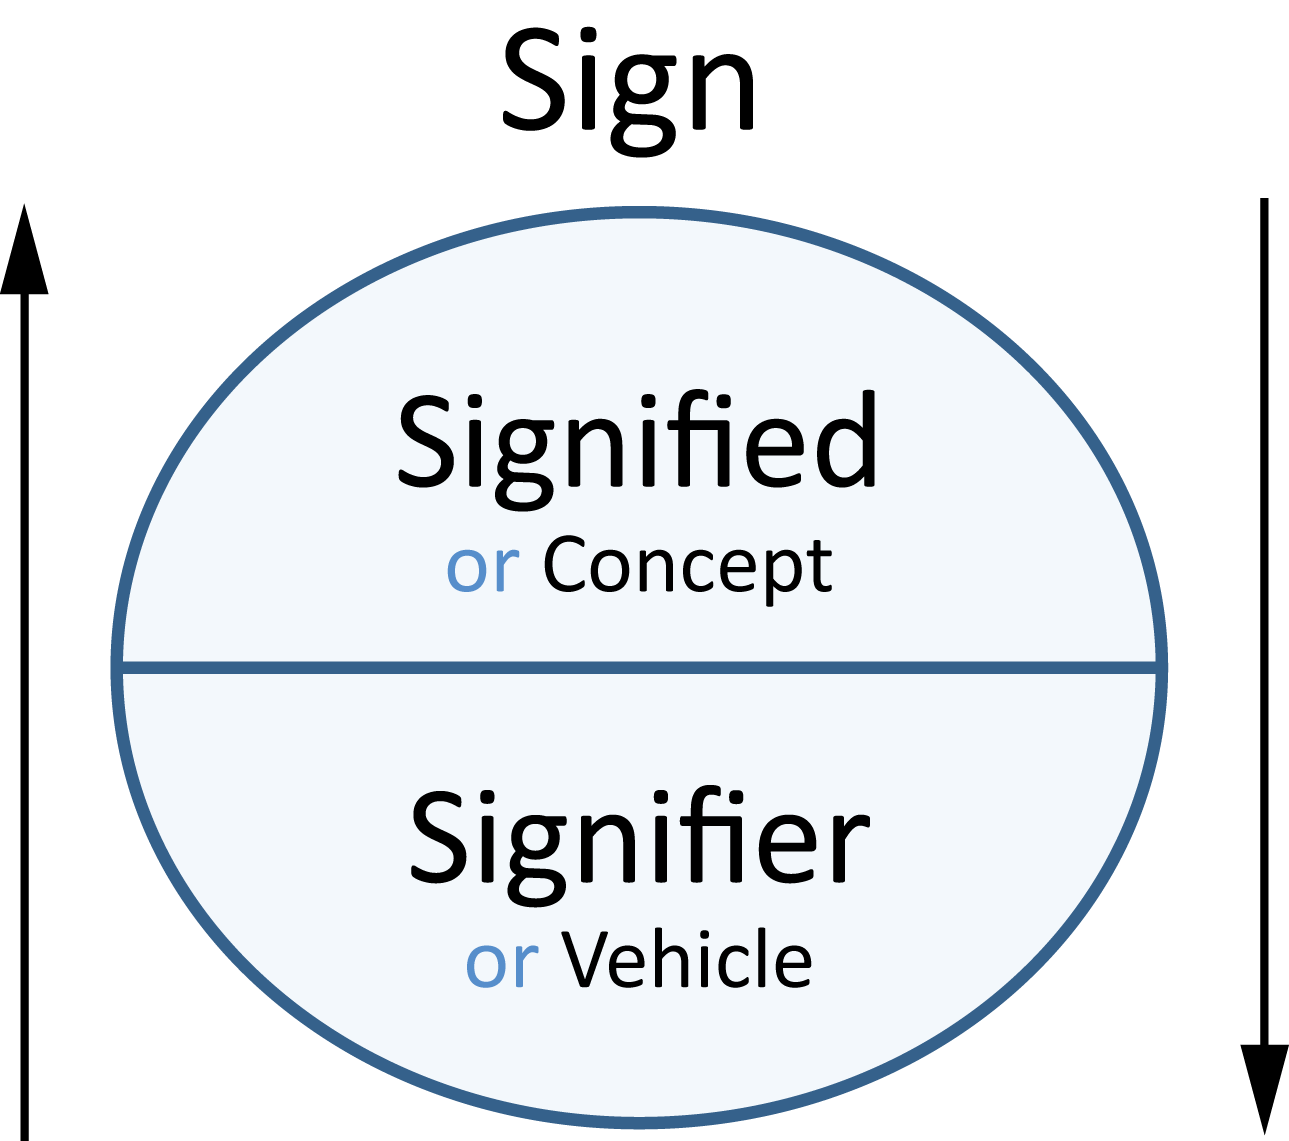
\includegraphics[width=.2\textwidth]{images/related-work-glyphs/Diadic.png}
\caption{The Dyadic Model of the Sign Notion of Ferdinand de Saussure~\cite{Saussure1983}.\label{fig:saussure}}
\end{figure}

In the Dyadic Model (Figure~\ref{fig:saussure}) introduced by Ferdinand de Saussure~\cite{Saussure1983} a sign is composed of the signifier (the sound pattern of a word, either in mental projection - as when we silently recite lines from a poem to ourselves - or in actual, physical realization as part of a speech act), and the signified (the concept or meaning of the word).

\begin{figure}[!t]
 \centering
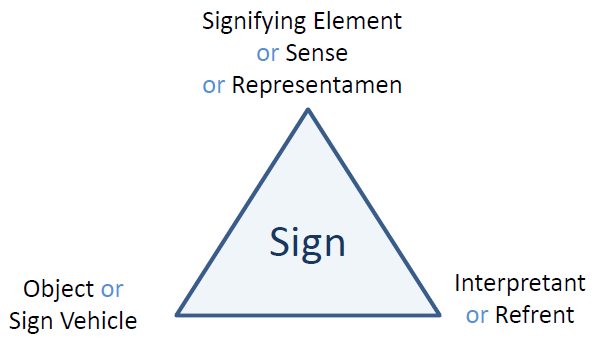
\includegraphics[width=.4\textwidth]{images/related-work-glyphs/Triadic.png}
\caption{The Structure of the Sign Notion (Triadic Model) of Charles Sander Peirce~\cite{Peirce1955}.\label{fig:peirce}}
\end{figure}  

%\subsubsection{The Triadic Model}
With its Triadic Model (Figure~\ref{fig:peirce}), Peirce~\cite{Peirce1955} viewed the symbol/index/icon triad as ``the most fundamental division of signs'', and the majority of semioticians continue to agree~\cite{Johansen1988}. 
Peirce thus defines ``semiosis'' as the process by which representations of objects function as signs. Semiosis is a process of cooperation between signs, their objects, and their ``interpretants'' (i.e. their mental representations). ``Semiotic'' (i.e. the science of signs) is the study of semiosis and is an inquiry into the conditions which are necessary in order for representations of objects to function as signs.

%\textbf{Should it be \emph{Symbolic Algebra}?}
%Algebraic semiotics is an attempt to formalize sign systems by defining an algebra that describes the set of signs possible in that system. 
%The promise of analyzing sign systems by describing them with an algebra is that we can draw conclusions about the sign system by mechanically applying the rules of algebraic manipulation, and analyzing the extent to which two different algebras are the same.
\subsubsection{Semiotic Systems: Algebra}

According to Saussure~\cite{Saussure1983} signs are always part of a formal system with a specific structure and relations. In its Semiotic Algebra Goguen~\cite{Goguen2003} devises a system to capture the systematic structure of a sign.
In Semiotic Algebra a sign is always divisible into subparts called \emph{sorts} (e.g., colour, location, size). Sorts may have a hierarchical structure with relationship such as inheritance or partial ordering between subsorts. 
Signs can be composed into more complex signs through constructor rules, functions that build new signs from other signs of given sorts plus additional parameters. Constructors express the whole/part relationship at the base of complex signs. 
Some sign constructors can be more important than others which gives rise to a priority partial ordering on the constructors of a given sort,  for example: the pollutants in a lake may be prioritised by their toxicity, to aid in the design of an appropriate visualization. 
The complexity of a sign is measured in term of a hierarchy of levels, with atomic signs at the lowest levels and complex sign built from signs at lower or same levels.


\subsubsection{Semiotic Systems: Grammar}
%Bertin's Taxonomy
Bertin~\cite{bertin83semiologyOfGraphics}  proposed the first and probably unique attempt at developing a syntax of visual signs based on formal rules. Bertin identified six visual primitives, or fundamental visual variables, which are at the basis of the construction of any graphics sign: size, colour hue, colour value, grain, orientation, and shape. Bertin rated each visual variable in function of the signified dataset, giving a rating of appropriate or inappropriate to each visual variable for numerical, ordinal, and categorical data. This laid down the grammatical rules of a syntax to guide the choice of appropriate forms of graphical representation. 
MacEachren~\cite{MacEachren:2004} proposed adding three extra variables based on advances in graphics technology (Figure~\ref{fig:MacEacVV}):
clarity (fuzziness) of sign vehicle components, resolution
(of boundaries and images), and transparency. He also provides a three-step rating for the full set of visual variables of good, marginal, and poor for use with numerical, ordinal, and categorical data.
Mackinlay~\cite{Mackinlay:1986:TOG} demonstrated the usefulness of such syntax of visual variables with his early implementation of an expert system for automating the design of graphical representations.

%eg. McGregor has a book entitled Semiotic Grammar

\section{Design Criteria and Guidelines}\label{sec:DesignCriteria}
Glyphs represent different data variables by a set of visual channels including shape, size, colour, orientation, etc.
It was a wide-spread opinion in the related research community for a long time that ``just'' knowing these basic principles of glyph-based visualization would suffice to its successful usage.
%these principles would suffice, % to utilize glyph-based visualizations successfully, 
More recently, however, it has been understood that only well designed glyphs are actually useful.
Visual channels such as colour~\cite{Christ75color} or size~\cite{Li10symbolSize} are more dominant and can help to focus the user's attention.
Other channels such as position, length, angle or slope can be measured and compared more accurately~\cite{ClevelandMcGill84Perception, Healey96preattentive}.
An effective glyph visualization should, therefore, carefully choose and combine different visual channels.
In this section, we discuss critical design aspects and guidelines for glyph-based visualization.


\subsubsection{Design Criteria}
According to Eco~\cite{Eco1979}, a general semiotic theory should include not only a theory of how codes may establish rules for systems of signification but a 
theory of how signs may be produced and interpreted to clarify aspects of communications.
In the work of Yousef~\cite{Yousef2001} five criteria have been proposed and empirically validated in the context of visual metaphors used in interface design.
The criteria proposed are referred to with the acronym of CARSE: contextual suitability, applicability of structure, representability/imagery, salience imbalance, prominence and emotional tone.

Context suitability, or relevance, indicates the extent to which the metaphorical sign resembles the source domain with respect to the context of use. 

Applicability of structure indicates the extent to which the proposed metaphorical sign is relevant to the new and unfamiliar concept that is being explained. 
The criteria can be regarded as the correspondence between the source and the target domain, in~\cite{Tourangeau1982} is referred to as ``Within-Domain Distance'' while Lakoff~\cite{Lakoff1995} calls it the ``Invariance Principle''. 

Representability/imagery indicates the ease with which the visual metaphor can be represented.

Salience imbalance refers to Ortony's~\cite{Ortony1993} statement that good metaphors are
the ones in which the source (vehicle) domain contains elements
or traits, which are highly explicit/prominent; at the same time
these traits are very subtle in the target (topic) domain. The visual representation should convey 
these salient source traits to the receiver. 

Emotional tone indicates the importance of emotions triggered by the
metaphor as one indicator of the semantic efficacy of the
function that is presented metaphorically.
In a recent study, Maguire et al. proposed a set of guidelines based on the literature of psychology and Bertin's categorisation of semantic relevance \cite{Maguire:2012:TVCG}.  These guidelines are:

\begin{figure*}[t]
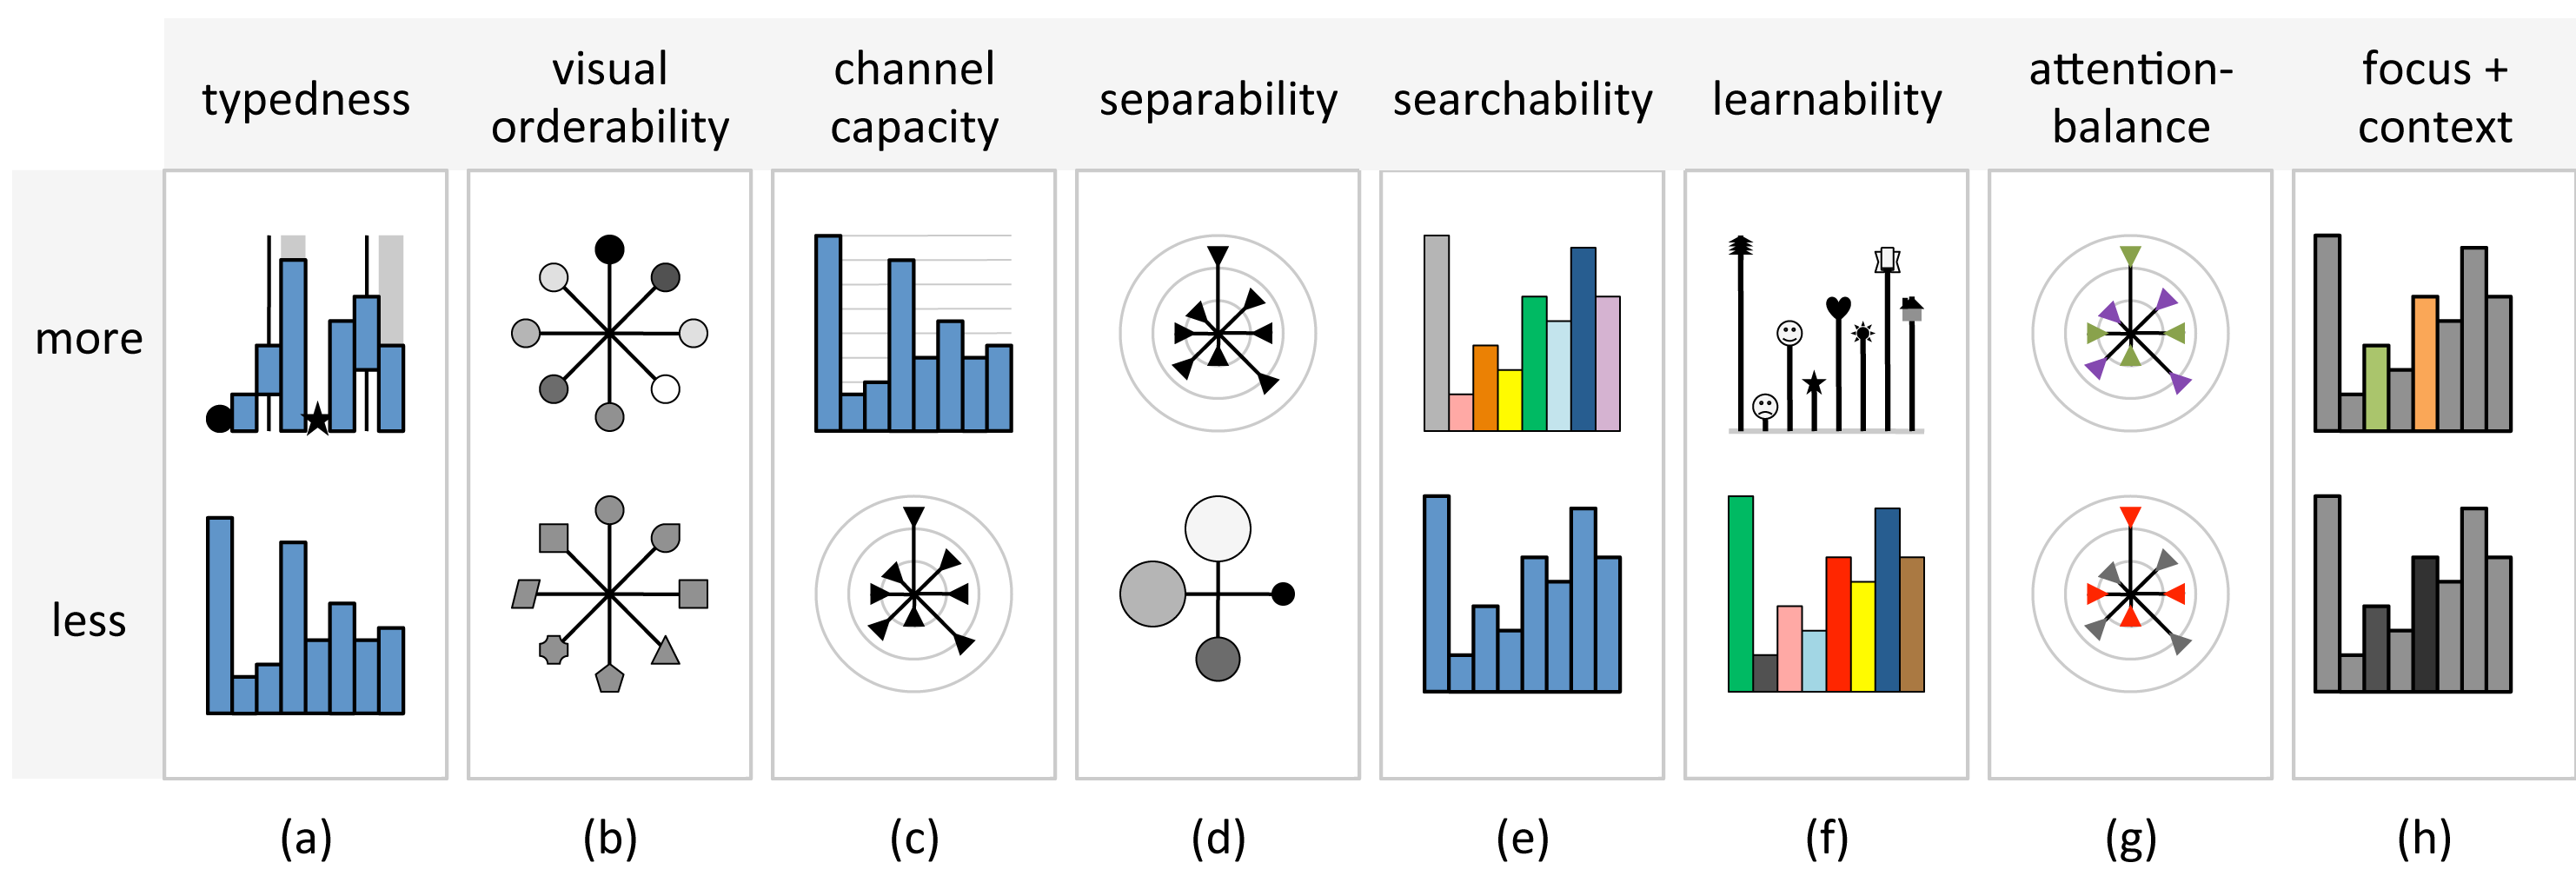
\includegraphics[width = \textwidth]{images/related-work-glyphs/designprinciples_ver2.png}
\caption{Glyph design criteria~\cite{chung13glyphSorting}.\label{fig:glyphSorting}}
\end{figure*}

A glyph is composed by a set of visual channels, each of which encodes a variable of a multivariate data record. Naturally the first criterion is that the visual channel should ideally be able to encode many valid values of that variable, or collectively, different visual channels of the glyph could encode many data records with different combinations of data values. However, this is not the only criterion, and in many cases, it may not even be the most important criterion. If the goal is to encode as many values as possible, one may be better off reading these values in text directly. Chung et al.~\cite{chung13glyphSorting} proposed eight criteria for glyph design in the context of sorting glyphs visually (Figure~\ref{fig:glyphSorting}). These are:

\renewcommand\theenumi {\alph{enumi}}
\begin{enumerate}
\item \emph{Typedness} -- This criterion refers to whether or not each visual channel in a glyph is appropriately selected to match with the data type of the variable to be encoded. Such data types may include, but not limited to: \emph{nominal}, \emph{ordinal}, \emph{interval}, \emph{ratio}, and \emph{directional}.
%
\item \emph{Visual Orderability} -- When a variable to be encoded is orderable, the corresponding visual channel should ideally be orderable visually (e.g., size, greyscale intensity, but not an arbitrary set of shapes). 
%
\item \emph{Channel Capacity} -- This refers to the number of values that may be encoded by a visual channel. Such a number is often affected by the size of a glyph and many perceptual factors (e.g., just-noticeable-difference, interference from nearby visual objects). 
%
\item \emph{Separability} -- When two or more visual channels are integrated into a compound channel, such as combining intensity, hue and saturation into a colour channel, the interference between different primitive channels should be minimised.
%
\item \emph{Searchability} -- This refers to the levels of ease when one needs to identify a specific visual channel within a glyph for a specific variable.
%
\item \emph{Learnability} -- This is often an important criterion in many applications. Ideally, a glyph design should be easy to learn, and easy to remember. There are many factors that may affect a visual design in this context, for instance, whether there are well-defined constructive rules, whether there are memorable metaphors, whether it is easy to guess, and so on.
%
\item \emph{Attention Balance} -- Different visual channels in a glyph will receive different levels of attention. Ideally, the levels of attention should correspond to the levels of importance of the variables. However, this is easier said than done as the relative importance of a variable is often undefined or may vary from tasks to tasks.
%
\item \emph{Focus and Context} -- This refers to the need to identify an individual visual channel under a certain interactive operation. For example, when a user select a certain variable as a sort key, it is desirable to highlight the corresponding visual channel so it stands out from other channels. 
\end{enumerate}

This is not an exhaustive list, and there are other design criteria, such as aesthetic appearance that also play an important role.


\subsubsection{Design Processes}
%In this section we will present some of the design principles that have assumed the \emph{guidelines} status in literature.
%These principles are at the base of information design.  
Petterson~\cite{Pettersson2010} introduces four categories of principles supporting the visual representation design process: 
\begin{itemize}
\item Functional Principles: focus, structure, clarity, simplicity, emphasis and unity;
\item Administrative Principles: accessibility, cost, ethics and quality;
\item Aesthetic Principles: harmony and aesthetic proportion;
\item Cognitive Principles: facilitating attention, facilitating perception, facilitating mental processing and facilitating memory.
\end{itemize}
For each category Petterson provides detailed guidelines on how to achieve the target result with the appropriate use of text, picture, layout and colour. 

Given the abundance of multivariate data, perceptual and cognitive efficiency is at the core of glyph-based visualization. 
Karve and Gleicher~\cite{Karve07} identify three considerations for the design of complex and compound glyphs: integral-separable dimension pairs, natural mappings and perceptual efficient encoding.
Integral-separable dimension pairs focus on the readability of multi-attribute glyphs and multi-glyphs displays, Karve and Gleicher~\cite{Karve07} argue that individual glyphs should combine as many separable visual attributes as possible and multi-glyph displays should be dense, juxtaposing related items, and employing repetitive design motifs that support inter-glyph comparison.
Natural mappings (e.g. use of metaphoric representations) focuses on the natural relationship between data and glyph features; a clear relationship between visual and data attributes enhances glyph usability.
Perceptual efficiency of the encoding focuses on the encoding of a continuous variable; horizontal bars on a shared positional scale are found to be the most accurate method followed in decreasing order of accuracy by interval length, slope, area, volume, and colour.  

\paragraph{Measurements and Norms}

%Criteria guiding metaphors designs eg. McDougall, Pettersson, Kennedy, Ng and Chan

If symbol design is to progress, we need
to know more about why some symbols are easier to use
than others.
A major obstacle facing researchers attempting to answer this question has been the difficulties in quantifying
symbol characteristics so that they can be experimentally controlled. A good way of controlling symbol characteristics
experimentally is to obtain subjective ratings of each characteristic.

Although there has been a long tradition
in psycholinguistic research of using normative ratings
to control item characteristics for words and pictures, no normative ratings for symbols have yet been
produced.
McDougall et al.~\cite{Mcdougall1999,Mcdougall2000} address the problem by providing normative ratings for five
symbol characteristics considered determinant in the development of easy to use and understand symbols: 
concreteness, visual complexity, meaningfulness, familiarity, semantic distance.

McDougall et al. highlights and investigates several interesting correlations between these five criteria. 
Concreteness, for example, (as opposed to abstraction) is somehow in opposition to visual complexity; concrete symbols tend to be more visually obvious because they depict objects, places, and people that are already familiar. In contrast, abstract symbols represent information using graphic features such as shapes, arrows and so on. One of the reasons why concrete symbols are more visually
obvious may simply be because the extra detail provided in concrete symbols makes them easier to comprehend. In contrast, however, design guidelines typically suggest
that the design of symbols or icons should be kept as simple as possible.
Other researchers have focused on the fact that concrete symbols are more meaningful than abstract symbols.

Semantic, or articulatory, distance is a measure of the closeness of the relationship between the symbol and what it is intended to represent.
A number of classification systems have been developed in order to attempt to characterise the different
relationships between symbols and their functions~\cite{Peirce1902}.

Familiarity reflects the frequency with which symbols are encountered. This property is thought
to be an important determinant of usability. It is evident that user performance improves dramatically as a result
of learning symbols and signs. 
%\textbf{TODO: Expand on this section.}
The effects of some symbol characteristics on performance, such as colour and concreteness, diminish as symbols become
more familiar but others, such as complexity, do not.

In~\cite{Mcdougall2000, Ng2008} the relationship between: concreteness/visual complexity, concreteness/meaningfulness and meaningfulness/familiarity/semantic distance were examined in detail using subjective rating methods. For each characteristic subjects had to choose bipolar adjectives based on a five-point scale to indicate their perception of an icon. 
Ng et al.~\cite{Ng2008} propose a review of the relationships among the same five characteristics together with a description of three types of measures used in literature to quantify such relationships:
\begin{itemize} 
\item subjective rating (as in~\cite{Mcdougall2000}); 
\item icon-based metric: the measure is obtained summing up the components of an icon, such as letters, lines, arrows and so on; 
\item automated visual measurement: the measure is a function of icon features  extracted via image analysis techniques such as edge-detection, perimeter determination, decomposition and so on.
\end{itemize}  
Other symbol characteristics present in literature are discriminability,
distinctiveness and configurality, however to provide a normative rating is a  much harder task since such characteristics can only be defined (and quantified) in relation
to the other symbols included in the display as a whole~\cite{Mcdougall2000}.


\begin{figure}[!th]
  \centering
  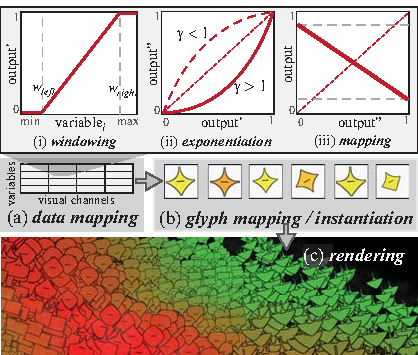
\includegraphics{images/related-work-glyphs/glyph-pipeline.pdf}
  \caption{A pipeline for creating glyphs [LKH09]: (a) Each data variable is subject to three stages of data mapping:
windowing, exponentiation and mapping.
(b) The data variables are mapped to the different visual channels of a glyph (e.g., upper/lower shape, size, and rotation) and used to instantiate the individual glyphs. (c) Finally, the glyphs are rendered in their spatial context.\label{fig:pipeline}}

\end{figure}
\begin{figure*}[!t]
  \centering
  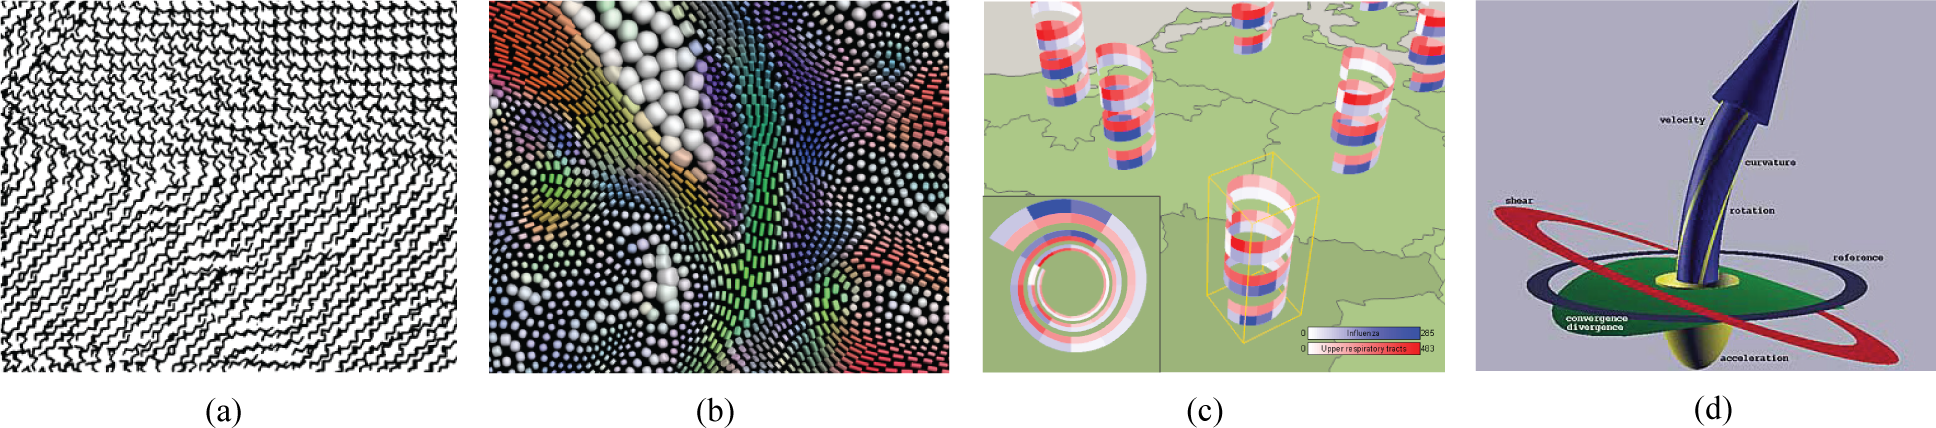
\includegraphics[width=\textwidth]{images/related-work-glyphs/sparse-vs-dense.png}
  \caption{Small simple glyphs vs.\ large and complex glyphs: 
  (a)~Stick figures form textural patterns~\cite{pickettGrinstein88iconic}. 
  (b)~Dense glyph packing for diffusion tensor data~\cite{kindlmannWestin06glyphPacking}. 
  (c)~Helix glyphs on maps for analyzing cyclic temporal patterns for two diseases~\cite{tominski05helix}.
  (d)~The local flow probe can simultaneously depict a multitude of different variables~\cite{deLeeuwVanWijk93probe}.}
\label{fig:sparseVsDense}
\end{figure*}
%\subsection{General Design Considerations and Guidelines}
%Use the available screen space between glyphs.

\subsection{Design and Usage Guidelines for Glyphs}
A number of design guidelines (marked with DGx in the following) for glyph-based visualization have been proposed~\cite{ward02glyphPlacement, ward08glyphs, ropinskiPreim08glyphTaxonomy, lie09glyphs, Ropinski11glyphs, Maguire:2012:TVCG}, and we review them in the following.
%In the context of information visualization,
Ward~\cite{ward02glyphPlacement} surveys glyph-based representations for information visualization
and presents a taxonomy for glyph placement.
% such as data- or structure-driven placement.
Ropinski et al.~\cite{ropinskiPreim08glyphTaxonomy, Ropinski11glyphs} propose a per\-ception-based glyph taxonomy for medical visualization.
Glyph-based visualizations are categorised according to: 
\begin{itemize}
\item ~\emph{pre-attentive} visual stimuli such as glyph shape, colour and placement, and 
\item ~\emph{attentive} visual processing, which is mainly related to the interactive exploration phase 
(e.g., changing the position or parameter mapping of a glyph).
\end{itemize}
In the context of medical visualization, the authors propose %a set of 
usage guidelines for glyphs, which are addressed later on.
%, for instance, that parameter mappings should focus the user's attention and emphasize important variates in the visualization.
%Also, glyph shapes should be unambiguous when viewed from different viewing directions.
%Kindlmann~\cite{kindlmann04superquad}, for example, use super\-quadric glyph shapes that fulfill the latter criterion.

%-------------------------------------------------------------------------
%\subsection{A pipeline for glyph-based visualization}
%-------------------------------------------------------------------------

Inspired by the work of Ropinski and Preim~\cite{ropinskiPreim08glyphTaxonomy},
Lie et al.~\cite{lie09glyphs} propose further guidelines for glyph-based 3D~data visualization.
Aligned with the visualization pipeline~\cite{hauserSchumann09pipeline},
the task of creating a glyph-based 3D~visualization is divided into three stages as shown in Figure~\ref{fig:pipeline}:
\begin{itemize}
\item ~during \emph{data mapping}, the data attributes of a record are remapped (to achieve, for example, some contrast enhancement) and mapped to the different visual channels of a glyph; 
\item ~\emph{glyph mapping} (or glyph instantiation) creates the individual glyphs, properly arranged across the domain; and 
\item ~during \emph{rendering}, the glyphs are placed in the resulting image, where one has to cope with issues such as visual cluttering or occlusion.
\end{itemize}
For each of these steps, the following sections discuss critical design aspects and guidelines for glyph-based visualization. %(Sec.~\ref{sec:dataMapping} to~\ref{sec:rendering}). %The different aspects are illustrated with a new glyph-based visualization of 3D~data.






Table~\ref{tab:scheme} illustrates different papers which are consistent with the design guidelines presented here.
The papers are also categorised according to the utilised visual channels, dimensionality of the visualization space, and density of glyph placement.
%The table is currently in a preliminary form, however, we will extend and carefully refine it in the final version of this survey.

\textbf{[DG1] Task-based choice of visualization space.}
Glyph-based visualization approaches vary with respect to whether they are constructed in a~2D or 3D~visualization space.
In case of abstract data such as census or financial data,
this decision is often dependent on the task at hand.
However, certain scenarios with 3D~volumetric or flow data inherently require
a 3D~visualization.
We think that it also makes sense to consider glyph-based visualizations, which are based on the placement of glyphs on 3D~surfaces~\cite{ropinski07surfaceglyphs} (called 2.5D in the following).


\textbf{[DG2] Task-based compromise between complexity and density.}
Glyph-based visualization approaches span a certain spectrum from dense arrangements of relatively simple shapes such as stick figures~\cite{pickettGrinstein88iconic} (Figure~\ref{fig:sparseVsDense}a) to individual instances of complex glyphs that reveal a lot of 
information (but only for few, selected places, Figures~\ref{fig:sparseVsDense}c and~d).
Additionally, we can differentiate visualization solutions according to 
which visual channels are varied according to the data,
and how many different values a glyph eventually represents.
Usually this number is not too large, often~2 to~4, but then also 
examples exist where dozens of values are represented (e.g., the local flow probe~\cite{deLeeuwVanWijk93probe} in Figure~\ref{fig:sparseVsDense}d).

\textbf{[DG3] Hybrid visualizations.}
Ropinski et al.~\cite{ropinskiPreim08glyphTaxonomy} suggest combining glyphs with other visualization techniques such as isosurfaces or volume rendering, 
which provide spatial context~\cite{ropinski07surfaceglyphs, crawfisMax93textureSplats}.
When glyphs are not placed in a dense way, the space between them can be used for additional information.
%provide spatial context 
%Spatial context can be provided should be exploited to provide spatial context~\cite{Ropinski11glyphs}.
Treinish~\cite{TreinishEffektiveWeather}, for example, visualizes multivariate weather data using colour contouring on vertical slices and isosurfaces that represent cloud boundaries.
At user-defined locations (vertical profiles), the wind velocity and direction are represented by a set of arrow glyphs.
Streamlines following the wind direction are seeded at each arrow.
Kirby et al.~\cite{kirby99multiValueFlow} use concepts from painting for visualizing 2D~flow. They combine different image layers with glyphs, elongated ellipses, and colour.
%-------------------------------------------------------------------------
\subsection{Data Mapping}
\label{sec:dataMapping}
%-------------------------------------------------------------------------
%\subsubsection{Visual Channel Ordering} 
Each dimension or variable of a data set will map to a specific graphical attribute. By modifying the order of dimensions while preserving the type of mapping, as many as N! alternate "views" of the data can be generated.  An important issue in using glyphs is to ascertain which ordering(s) will be most supportive of the task at hand.  Several possibilities exist, beyond random ordering or the order in which the variables were originally stored~\cite{ward08glyphs}:
\begin{itemize}
\item \textbf{Correlation-driven.} Many researchers have proposed using correlation and other similarity measures to order dimensions for improved visualization~\cite{bertin83semiologyOfGraphics,Ankerst:1998,Friendly:2003,Borg:1992}.  These orderings help reveal clusters of similar variables, outlier records, and gradual shifts in relationships between variables.
\item \textbf{Complexity and Symmetry-driven.} Gestalt principles indicate we have a preference for simple shapes, and we are good at seeing and remembering symmetry.  In~\cite{Peng04dimensionReordering} the shapes of star glyphs resulting from using different dimension orders were evaluated for two attributes: monotonicity (the direction of change is constant) and symmetry (similar ray lengths on opposite sides of the glyph).  The ordering that maximised the number of simple and symmetric shapes was chosen as the best.  User studies showed improved performance with complexity and symmetry optimised orderings.
\item \textbf{Data-driven.} Another option is to base the order of the dimensions on the values of a single record (base), using an ascending or descending sort of the values to specify the global dimension order.  This can allow users to see similarities and differences between the base record and all other records.  For example, sorting the exchange rates of 10 countries with the U.S. by their relative values in the first year of the time series exposes a number of interesting trends, anomalies, and periods of relative stability and instability (Figures~\ref{fig:mWard1}  and~\ref{fig:mWard2}).  
\item \textbf{User-driven.} As a final strategy, we can allow users to apply knowledge of the data set to order and group dimensions by many aspects, including derivative relations, semantic similarity, and importance.  Derivative relations mean that the user is aware that one or more dimensions may simply be derived through combinations of other dimensions. Semantic similarity indicates dimensions that have related meanings within the domain.  
\end{itemize}
Finally, some dimensions are likely to have more importance than others for a given task, and thus ordering or assigning such dimensions to more visually prominent features of the glyph will likely have a positive impact on task performance. 
%When representing a data variate it can be
In order to optimally represent a data variable using a visual channel of the glyph, the corresponding data range should be normalised, for instance, to the unit interval~\cite{Ropinski11glyphs, ward02glyphPlacement, lie09glyphs}.
The remapped data attributes parameterize the visual appearance of a glyph.
Ropinski et al.~\cite{ropinski07surfaceglyphs}, for example,
use an interface similar to a transfer function editor for mapping a data attribute to a visual channel of the glyph.
\begin{figure}[!t]
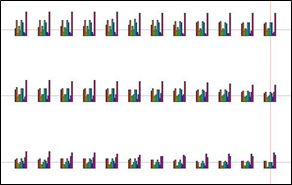
\includegraphics[width=\columnwidth]{images/related-work-glyphs/mWard1.png}
\caption{The figure shows monetary exchange rates over 3 years using random ordering.\label{fig:mWard1}}
\end{figure}
\begin{figure}[!t]
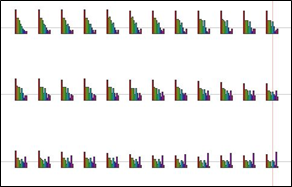
\includegraphics[width=\columnwidth]{images/related-work-glyphs/mWard2.png}
\caption{In this figure, the dimensions are sorted based on the first record.  Gradual changes and anomalies are much easier to perceive.\label{fig:mWard2}}
\end{figure}

\begin{table*}%
\centering
  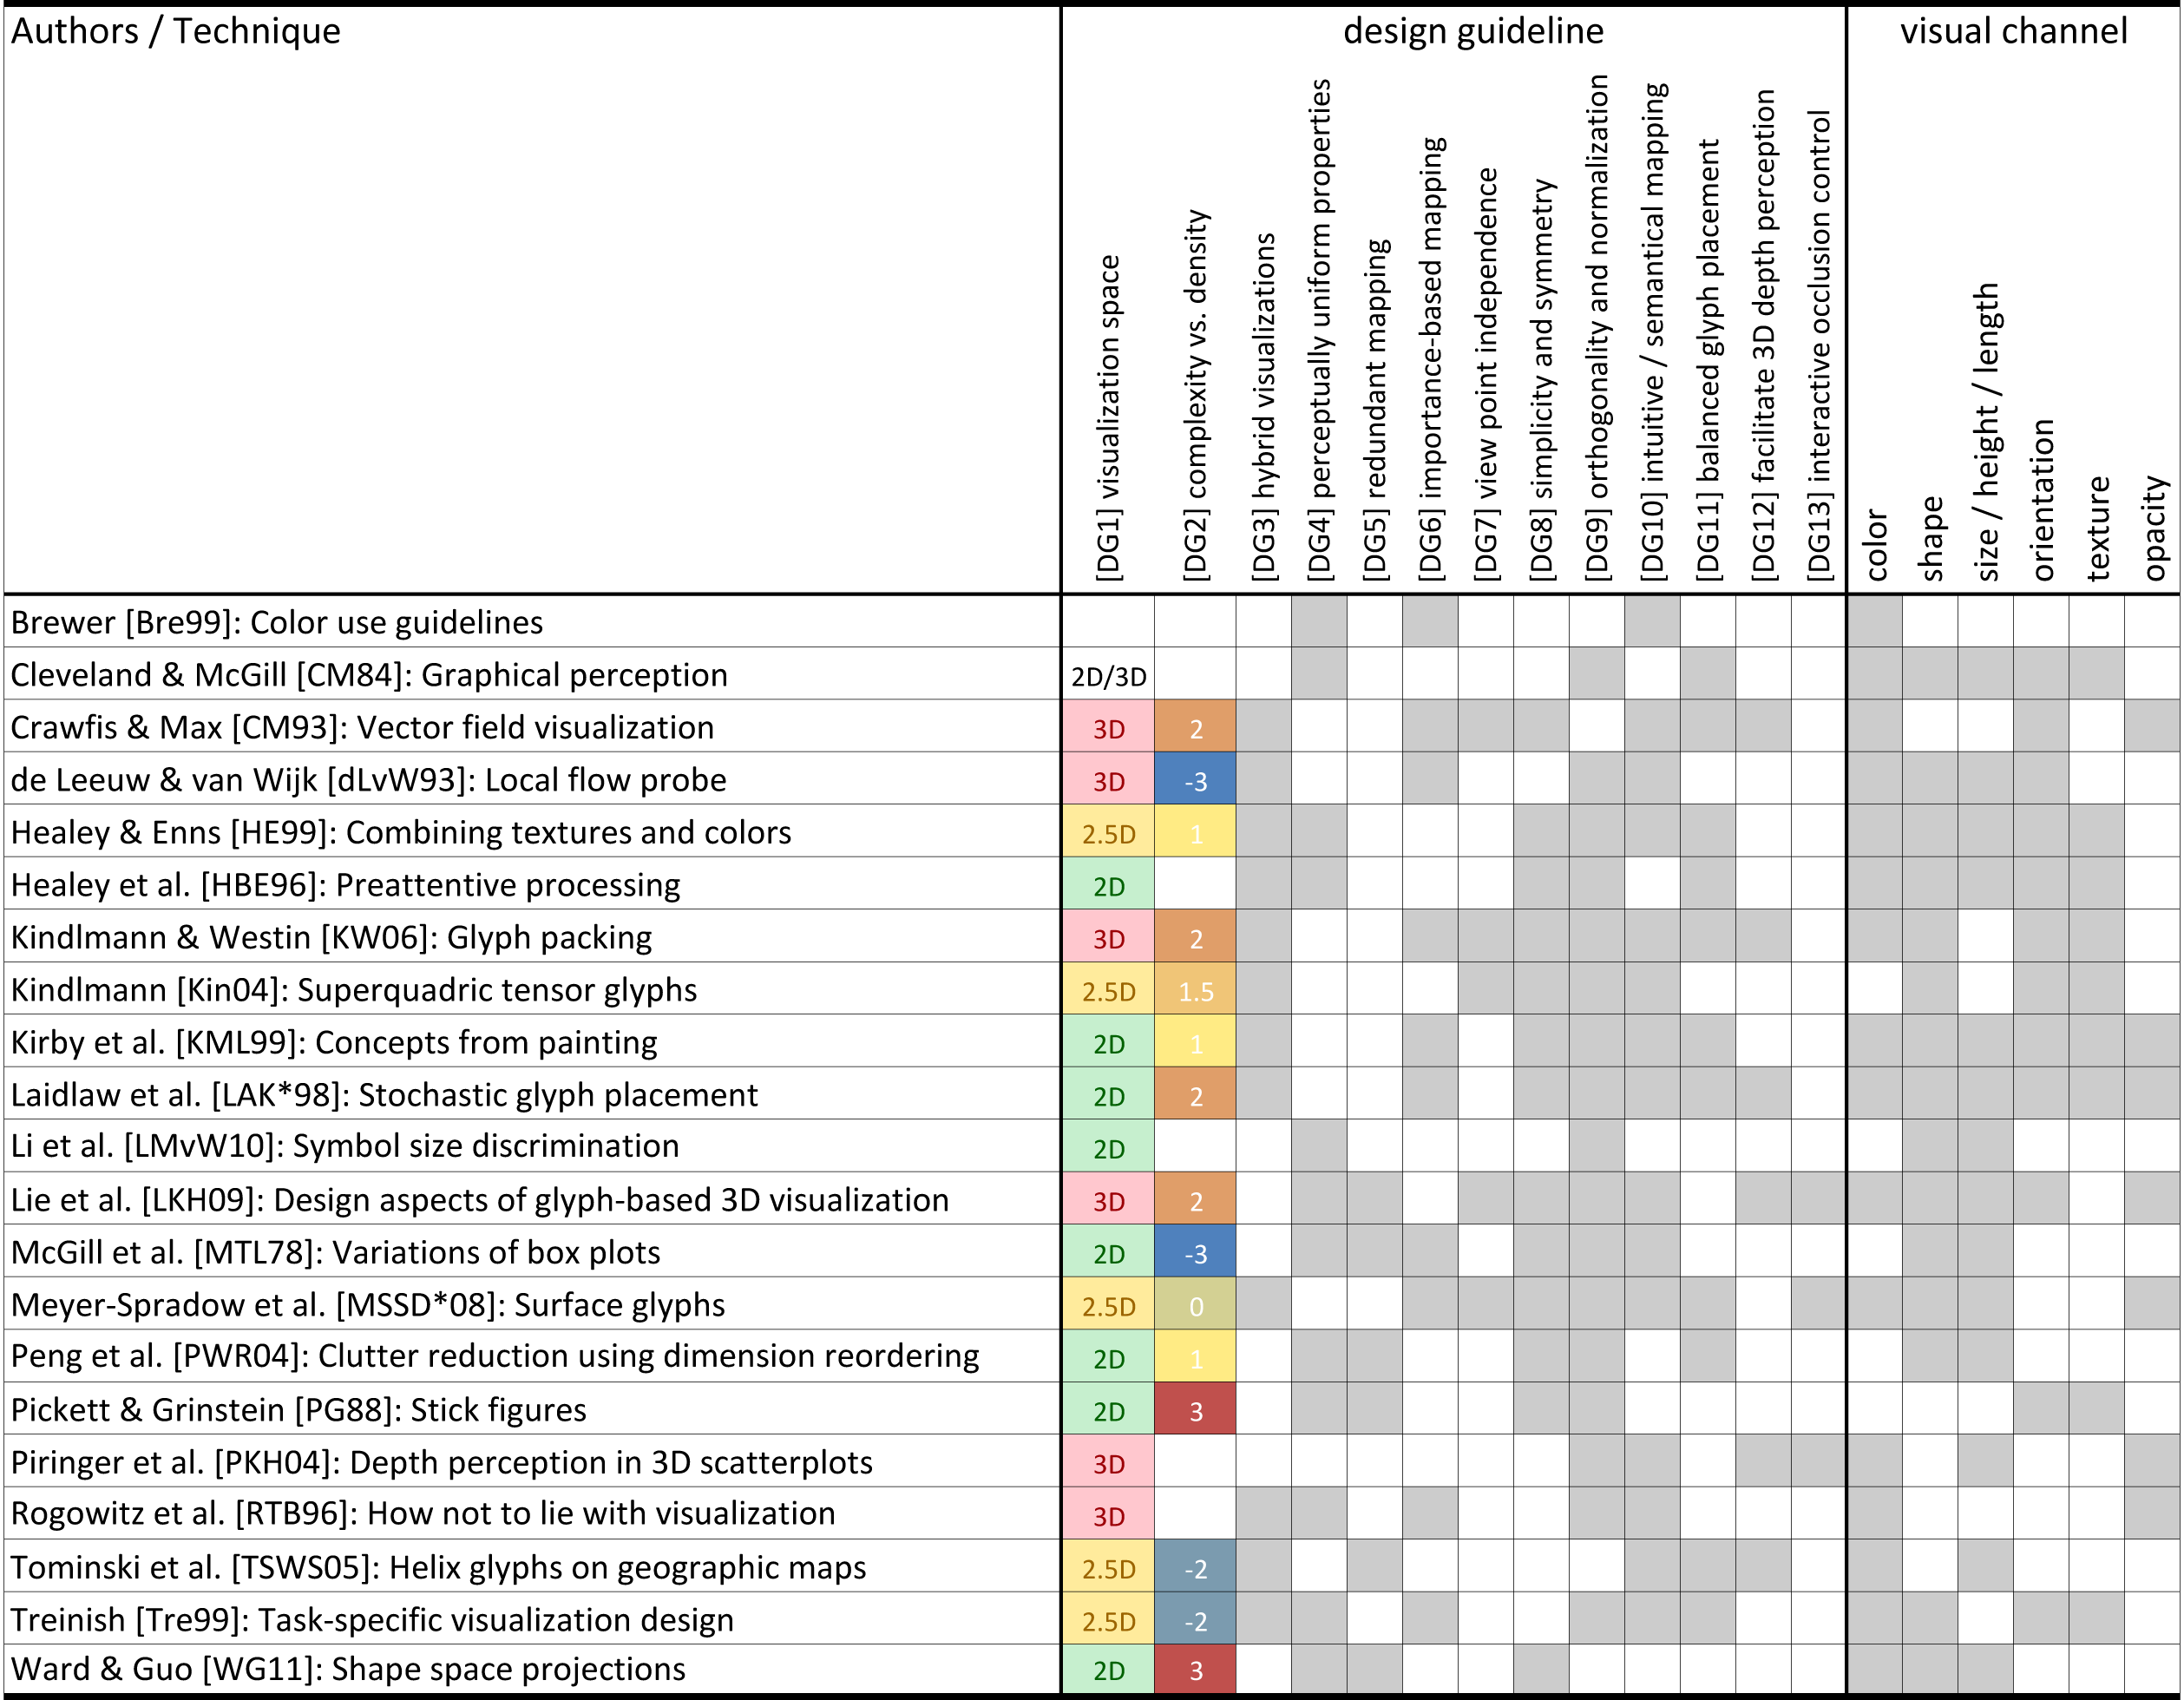
\includegraphics[width=\textwidth]{images/related-work-glyphs/table1.png}
\caption{Categorisation of glyph-based approaches according to design guidelines, visualization space and visual channels. In DG2, the approaches span a spectrum from individual instances of complex glyphs (-3) to dense arrangements of relatively simple shapes (+3).}
\label{tab:scheme}
\end{table*}
Lie et al.~\cite{lie09glyphs} propose three consecutive steps for the 
data mapping stage.
First, the data values within a user-selected data range~$[w_\mathit{left}, w_\mathit{right}]$ are mapped to the unit interval (Figure~\ref{fig:pipeline}a (i)).
Values outside this range are clamped to~$0$ or~$1$, respectively.
Consequently, the contrast of the visualization can be enhanced with respect to a range of interest (sometimes called \emph{windowing}).
A linear mapping would be a natural choice for this step, but also other forms of mapping could be considered, such as a discontinuous mapping.
%A natural default choice for this step would be a linear map between $[w_\mathit{left}, w_\mathit{right}]$ and~$[0, 1]$, 
Another option would be a ranking-based mapping where the data is sorted first and each discrete value (or bin) is then shown differently, for example, using different shapes such as a triangle, circle, or star~\cite{stolte02polaris}.
After the windowing, the contrast of a data variable can be further enhanced using an optional exponential mapping~$e(x)=x^\gamma$.
%While 
Using a value~$\gamma \in ]0, 1[$, smaller values are represented more prominently (see the dashed red curve in Figure~\ref{fig:pipeline}a (ii)).
In contrast, larger values are emphasised with $\gamma > 1$.
Since an exponential mapping can be hard to interpret, it should not be used as a default mapping.
It can rather be applied when the user is interactively exploring the visualization, for instance, by modifying the parameter mappings to focus of different portions of the data.
% can be applied in order to further enhance the contrast on the one or the other end of the spectrum.
Finally, a third mapping step enables the user to restrict or transform the output range that should be depicted by a visual channel.
Using a reverted mapping, for instance, smaller values, which are possibly more important to the user, are depicted in an enhanced style while larger values are de-emphasised.
Consequently, also semantics of the data variables can be considered, which is an important guideline when mapping a data variable to a visual channel of a glyph~\cite{ward02glyphPlacement, Ropinski11glyphs}.

%Ward~\cite{ward08glyphs} also discusses different strategies for ordering data
%variables such as correlation-driven, symmetry-driven, data-driven, and user-driven.

%-------------------------------------------------------------------------
\subsection{Glyph Mapping / Instantiation}
%-------------------------------------------------------------------------
%\emph{Alternatively called Glyph Instantiation/Generation. Check this!}

During glyph mapping the individual glyphs are created by representing the data variables with different visual channels of a glyph. During this step, the glyphs are also properly arranged across the domain. 
In the following, we discuss general design guidelines during this mapping stage as well as guidelines related to glyph shape and appearance.
%creates the individual glyphs, properly arranged across the domain

\textbf{[DG4] Perceptually uniform glyph properties.}
When mapping a data variable to a glyph property, equal distances in data space should be perceived equally as well.
This is an important guideline for glyph design, and it was originally developed for colour maps~\cite{Rogowitz96lieWithVis}.
The box~plot~\cite{mcGill78boxPlots}, for example, uses position and height of the box~/ whiskers to encode minimum and maximum value, median, and other quartile information of a data distribution.
%Human perception can measure this properties more accurately tha
A negative example in this context would be mapping a data variable to the radius of a circle. The circle's area then increases quadratically with respect to the radius (instead of linearly).
Li et al.~\cite{Li10symbolSize} study the perception of symbol size, which is assumed to be the second dominant visual channel (after colour~\cite{Christ75color}).
Their experiments suggest that the perception of size can be best represented by a power law transformation. % \textbf{[Also study of lightness (PacificVis)?]}
Another negative example would be the usage of a rainbow colour map, which is not perceptually uniform and does not have a perceptual ordering~\cite{BorlandTaylor07rainbowColormap}.
%This guideline can be easily applied to glyph design, when mapping different data variates to glyph properties.
%one of the most important guidelines 
%Human perception can measure certain properties more accurately than others.
%Schulz and Kindlmann~\cite{SchultzKindlmann10symmetricTensors} discuss th
%This guideline can be easily applied in glyph design, when mapping different data variates to glyph properties.
%Visual properties such as position or length can be measured more accurately than area or size~\cite{}

\textbf{[DG5] Redundant mapping of variables.}
According to Ward \cite{ward08glyphs}, there are three different mappings: 
\begin{itemize}
	\item a~one-to-one mapping assigns each data variable to a different visual channel of the glyph;
 \item a~one-to-many mapping makes use of redundancies by mapping a data variable to multiple glyph channels.  Such a mapping can reduce the risk of information loss by encoding important variables multiple times, which is also an important guideline for glyph design~\cite{lie09glyphs, Ropinski11glyphs}.
%\textbf{[Important properties can, moreover, be mapped to multiple glyph properties in order to reduce the risk of information loss.]}
 \item a~many-to-one mapping represents multiple data variables by the same kind of visual channel, for example, the height of bars in a histogram or profile glyph.  Such a mapping is useful when comparing the different data variables for a data element~\cite{ward08glyphs}.
%The most common mappings are one-to-one and one-to-many mappings.
\end{itemize}

\textbf{[DG6] Importance-based mapping.}
According to Ropinski et al.~\cite{Ropinski11glyphs},
%A number of guidelines address the mapping of a data variate to a visual channel of a glyph.
important variables should be enhanced in the visualization, for instance, by using a redundant mapping (compare to the previous guideline).
% in order to reduce the risk of information loss~\cite{lie09glyphs}.
Moreover, the mapping should guide the user's \emph{focus of attention}, e.g., using more prominent visual stimuli such as colour, size or opacity to encode relevance.
Ropinski et al.~\cite{ropinski07surfaceglyphs}, for example, use surface glyphs to show data from positron emission tomography~(PET).
An inverse mapping is used, which maps low PET~activity to thick and high PET~activity to thin glyphs.
Consequently, interesting regions with reduced activity are shown in an enhanced style.
%Also the glyph shape is a prominent visual 
Maguire et al propose an algorithmic approach to importance-based mappings~\cite{Maguire:2012:TVCG}. Their algorithm builds a taxonomy (a hierarchical classification) from a list of qualitative terms grouped into classification schemes. The higher up some classification scheme is in the taxonomy (determined algorithmically and based on term use for instance), the stronger the visual channel to represent that scheme will be.



\subsubsection{Shape Design}
One of the most prominent visual channels of a glyph is its shape.
Ropinski et al.~\cite{Ropinski11glyphs} distinguish between \emph{basic glyph shapes} such as variants of superquadrics~\cite{barr81} (sphere, torus) and \emph{composite shapes} that combine multiple basic shapes.  Since basic shapes can be perceived pre-attentively the authors argue that they should be used to convey the most important information.
Composite glyphs, on the other hand, are interpreted in the exploration phase and are usually not pre-attentive, i.e., they are analysed sequentially.
Chernoff faces~\cite{Chernoff73faces}, for instance, represent data variables by different features of a cartoon face (e.g., shape of the face; 
size and position of eyes, nose, and mouth; curvature of the mouth).
The Glyphmaker~\cite{Ribarsky94glyphMaker} provides a user interface that enables non-programmers to map data variables to the different properties of a glyph such as position, colour, shape, overall size and transparency.
Kraus and Ertl~\cite{KrausErtl01customizedGlyphs} propose a similar tool for scientific data.
%[example ; %Chernoff faces-]

%\textbf{2D vs.\ 3D glyphs:}
\textbf{[DG7] View point independence:}
Glyph shapes should be unambiguously perceivable independent of the viewing directions~\cite{Ropinski11glyphs}.
When using 3D~glyph shapes, one has to account for possible distortions introduced when viewing the glyph from a different point of view.
Lie et al.~\cite{lie09glyphs}, therefore, suggest to use 2D~billboard glyphs in order to avoid this problem. %
%\footnote{A billboard is a planar structure placed in a 3D~scene, which automatically adjusts its orientation such that it always faces the observer.}
In certain scenarios, however, it makes sense to use 3D~glyphs, for example, when they have a semantic meaning. Such an example would be arrow glyphs that depict a flow field~\cite{crawfisMax93textureSplats}.
Kindlmann~\cite{kindlmann04superquad} use super\-quadric glyph shapes that fulfill DG7.
%\textbf{[or showing the principle direction in DTI data]}.
For composite shapes, Ropinski et al.~\cite{Ropinski11glyphs} distinguish between directional and non-directional glyphs.

\textbf{[DG8] Simplicity and Symmetry:} According to Gestalt laws~\cite{ware04infoVis}, simple and symmetric shapes facilitate the perception of visual patterns.
Also, simple glyph shapes enhance the detection of minor shape changes as well as outliers~\cite{ward08glyphs}.
Peng et al.~\cite{Peng04dimensionReordering}, for instance, automatically reorder the data-to-property mapping for generating more symmetric and simple star glyphs.
Lie et al.~\cite{lie09glyphs} propose horizontally symmetric glyphs that are based on superellipses, which should facilitate the mental reconstruct of glyph parts that are occluded.
%Ward discusses dimension ordering app
%Symmetrie that ease the reconstruction of occluded parts of the glyph.
%[Ward suggests dimension ordering that creates symmetric glyph shapes~\cite{ward08glyphs}.
%Perception research shows that humans prefer simple and symmetric shapes.]


In the following, additional guidelines for shape design are discussed in relation to other visual properties.
%\textit{We should have a two-liner here explaining that it isn't so that there's only one DG wrt. shape design, but instead other DGs -- maybe we can even reproduce their codes here -- associate with shape design, also.}

%\textbf{Guideline:} 

\subsubsection{Other Visual Properties / Glyph Appearance}

Pre-attentive visual stimuli such as position, width, size, orientation, curvature, colour (hue), or intensity are a powerful way to represent data~\cite{ClevelandMcGill84Perception, Healey96preattentive}.
% Multiple data values can be simultaneously represented %at a spatial location using 
These visual channels are rapidly processed by our low-level visual system and can thus be used for the effective visualization of large data.
%items~\cite{fekete02million}.
Special care is required, however, if several such stimuli are combined---the result may not be pre-attentive any more.
Healey and Enns~\cite{healey99largeDatasetsAtGlance} propose simple texture patterns and colour to visualize multivariate data.
Different data variables are encoded in the individual elements of a perceptual texture %(pexels) 
using equally distinguishable colours and texture dimensions such as element density, regularity and height.
Groups of neighboring elements form texture patterns that can be analysed visually.

%\textbf{Biases in Glyph Mapping:} 
Ward~\cite{ward08glyphs} identifies different biases that are introduced when mapping a data variable to a glyph property.  The first kind of biases are related to human \emph{perception}.
Different properties of a glyph can be perceived and related with varying accuracy. Cleveland and McGill~\cite{ClevelandMcGill84Perception} identify different visual channels and perform perceptual experiments.
The visual channels are ordered based on how accurately they can be perceived: 1)~position along a common scale; 
2)~position along non-aligned scale; 3)~length, angle or slope; 4)~area; 
5)~volume or curvature; 6)~shading or colour saturation.
Moreover, adjacent properties of a glyph are easier to relate and compare than nonadjacent (Ward calls these \emph{proximity}-based biases~\cite{ward08glyphs}).
Finally, data variables mapped to semantically or perceptually \emph{grouped} glyph properties (e.g., the ears or eyes in Chernoff faces~\cite{Chernoff73faces}) are easier to distinguish than variables mapped to non-related features.

\textbf{[DG9] Orthogonality and Normalization:}
When designing glyphs, it is especially important to consider how different glyph properties interact with each other and thereby possibly distort the interpretation (compared to channel composition~\cite{Maguire:2012:TVCG}).
A challenge in this context is the \emph{orthogonality}~\cite{lie09glyphs} of the different glyph components, meaning that it should be possible to perceive each visual cue independently (or to mentally reconstruct the depicted data variables as suggested by Ropinski et al.~\cite{Ropinski11glyphs}).
Moreover, one has to account for %biases and 
distortions introduced by the different glyph properties. When using, for example, glyph shape to represent a data variable this affects the area (size) of the glyph as well.
Accordingly, such effects should be \emph{normalised} against each other~\cite{lie09glyphs}. 
In the previous example, the overall glyph size could thus be altered in order to compensate for the changes introduced by variations in shape.
However, it is not always easy to design a glyph-based visualization such that the different data-to-property mappings are independent and do not influence each other (e.g., the interpretation of shape details is usually influenced by the size of the glyph).


\textbf{[DG10] Intuitive mapping based on semantics.}
Semantics of the data should be incorporated in the glyph mapping~\cite{ward08glyphs, lie09glyphs, Ropinski11glyphs,Maguire:2012:TVCG}.
Crawfis and Max~\cite{crawfisMax93textureSplats}, for instance, combine small coloured vector glyphs depicting wind velocity with contour surfaces representing cloudiness.
%Crawfis and Max~\cite{crawfisMax93textureSplats}, for example, combine small colored vector glyphs depicting wind velocity with contour surfaces representing cloudiness.
%, for instance, encoding flow directions with arrow glyphs. 
Another example would be to represent temperature with a diverging colour map~\cite{brewer99colorGuidelines}, where white is used to indicated 0$^\circ$C, blue indicates minus and red plus degrees.
%1)~perception-based (\eg, some attributes easier to measure and compare~\cite{cleveland93visualizingData}, \eg, length easier than orientation, size or color); 
%2)~proximity-based (\eg, easier to compare adjacent features),

%Our glyph is horizontally symmetric which should make it easier to mentally reconstruct the glyph shape when parts of it are occluded.
%It can also
%In Fig.~\ref{fig:glyphContr}a--d, an increasing number of variates is represented by our proposed glyphs.
%The use of glyph size and aspect ratio should be handled with care, since these glyph properties may distort the interpretation of others.
%Size can be used, for instance, to focus on important aspects of the data (similar to a focus+context style).
%Fig.~\ref{fig:glyphMap} shows how the upper/lower glyph shape represent a data variate by changing from a star (small value), to a diamond, to a circle, and a box representing a large value.
%Since the changes in shape affects the area (size) of the glyph,
%we suggest to \emph{normalize} these effects against each other.
%Accordingly, the overall glyph size is altered in order to compensate for these implicit changes.
%Another design guideline is the use of \emph{redundancies}.
%Our glyph is horizontally symmetric which should make it easier to mentally reconstruct the glyph shape when parts of it are occluded.
%Important properties can, moreover, be mapped to multiple glyph characteristics in order to reduce the risk of information loss.
%When designing glyphs, it is especially important to consider how different glyph properties interact with each other and thereby possibly distort the interpretation (compare to glyph size and aspect ratio).


